\documentclass[../../../analisi-dei-requisiti.tex]{subfiles}

\begin{document}

\subsubsection{AUC13: Eliminazione account}%
\label{subs:AUC13}

\begin{figure}[H]
  \centering
  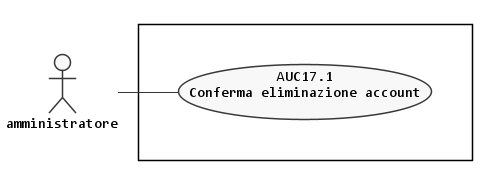
\includegraphics[width=100mm]{eliminazione-account-wa-conferma.png}
  \caption{AUC13: Eliminazione account}%
  \label{fig:AUC13}
\end{figure}

\begin{description}
  \item[Codice:] AUC13;
  \item[Titolo:] Eliminazione account;
  \item[Attori primari:] amministratore;
  \item[Precondizione:] deve essere stato selezionato l'\glossario{account} da eliminare, che deve esistere in \emph{Stalker};
  \item[Postcondizione:] l'account selezionato è stato eliminato;
  \item[Scenario principale:]
  \begin{enumerate}
    \item sorge la necessità di eliminare un account.
  \end{enumerate}
\end{description}

\subsubsection{AUC13.1: Conferma eliminazione account}%
\label{subs:AUC13.1}
\begin{description}
  \item[Codice:] AUC13.1;
  \item[Titolo:] Conferma eliminazione account;
  \item[Attori primari:] amministratore;
  \item[Precondizione:] l'utente deve aver selezionato l'account;
  \item[Postcondizione:] l'account viene eliminato;
  \item[Scenario principale:]
  \begin{enumerate}
    \item l'amministratore conferma l'eliminazione di un account.
  \end{enumerate}
\end{description}
\end{document}
